\section{Multimaps}
\begin{itemize}
    \item Sind ungeordnet
    \item Methoden:
    \begin{itemize}
        \item find(k): Liefert Entry zum Key k oder null
        \item findAll(k): Liefert Collection mit allen Entries zu Key k
        \item insert(k,o) neue Entry mit Key k und Wert o
        \item remove(e) entfernt Entry e und gibt zurück
    \end{itemize}
\end{itemize}

\subsection{Geordnete Multimap}
\begin{itemize}
    \item Keys folgen einer vollständigen Ordnungsrelation
    \item Neue Methoden:
    \begin{itemize}
        \item first(): liefert erste Entry in Multimap
        \item last(): liefert letzte Entry in Multimap
        \item successors(k): liefert Iterator über Entries mit Schlüssel grösser oder gleich k
        \item predecessors(k): liefert Iterator über Entries mit Schlüssel kleiner oder gleich k
    \end{itemize}
\end{itemize}

\section{Binäre Suche}
Bei einer Multimap, realisiert als array-basierte Sequenz, sortiert nach Key, gilt für die Operation find(k):\\
\begin{itemize}
    \item bei jedem Schritt wird die Anzahl der Kandidaten halbiert
    \item terminiert nach O(log n) Schritten
\end{itemize}
\begin{center}
    \vspace{-4pt}
    \includegraphics[scale=.18]{graphic/01 BinarySearchTrees/Binäre Suche.png}
    \vspace{-8pt}
\end{center}

\section{Suchtabelle}
\begin{itemize}
    \item Multimap, mithilfe einer sortierten Sequenz implementiert
    \item Entries der Multimap werden in einer Array-basierten Sequence abgespeichert, sortiert nach Schlüssel.
    \item Performance:
    \begin{itemize}
        \item find: 0(log n) falls mit Binärbaum umgesetzt
        \item insert: O(n) $\rightarrow$ im worst-Case alte Entry um 1 verschieben
        \item remove: O(n) wie insert
    \end{itemize}
    \item nur dann effektiv, wenn die Multimap klein ist und vor allem Such-Operationen ausgeführt werden
\end{itemize}


\section{Binärer Such-Baum}
\begin{center}
    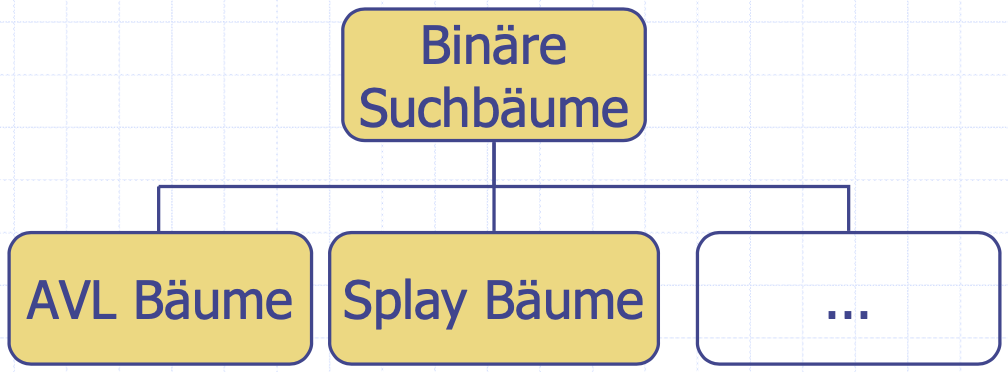
\includegraphics[scale=.15]{graphic/01 BinarySearchTrees/Ubersicht.png}
    \vspace{-4pt}
\end{center}
\begin{itemize}
    \item Binärer Baum, welcher Keys in seinen internen Knoten speichert
    \item Die Inorder-Traversierung besucht die Keys in nicht absteigender Folge
    \item Externe Knoten (Blatt-Knoten) speichern keine Daten
\end{itemize}

\subsection{Suche}
\begin{itemize}
    \item Suche nach dem Key k beginnen bei Root
    \item nächste Knoten ist, hängt vom Resultat des Vergleiches von k mit dem Key des aktuellen Knotens ab
    \item Wenn ein Blatt erreicht $\rightarrow$ Key nicht gefunden $\rightarrow$ geben v zurück
\end{itemize}
\begin{center}
    \vspace{-8pt}
    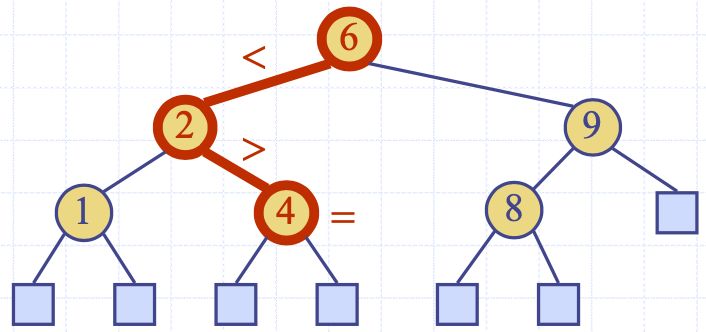
\includegraphics[scale=.3]{graphic/01 BinarySearchTrees/suche.png}
\end{center}
\begin{lstlisting}
Algorithm TreeSearch(k, v)
    if T.isExternal (v)     //Bsp: t.left(8)
        return v
    if k < key(v)           //Bsp: key(6)
        return TreeSearch(k, T.left(v))
    else if k = key(v)      //Bsp: key(4)
        return v
    else { k > key(v) }     //Bsp: key(2)
        return TreeSearch(k, T.right(v))
\end{lstlisting}

\subsection{Einfügen}
\begin{itemize}
    \item suchen wir zuerst den Key k
\end{itemize}
\subsubsection{Fall 1:}
\begin{itemize}
    \item k noch nicht im Baum und w ist Blatt, welches mit der Suche gefunden wird
    \item fügen k beim Knoten w ein und expandieren w in einen internen Knoten
\end{itemize}
Beispiel: insert(5)
\vspace{-8pt}
\begin{multicols}{2}
    \includegraphics[scale=.25]{graphic/01 BinarySearchTrees/einfügen1.1.png}
    %\columbreak
    \includegraphics[scale=.25]{graphic/01 BinarySearchTrees/einfügen1.2.png}
\end{multicols}
\vspace{-8pt}

\subsubsection{Fall 2:}
\begin{itemize}
    \item k ist schon im Baum vorhanden
    \item im linken Teilbaum von k wird weitergesucht bis auf Blattknoten w stösst
    \item fügen k beim Knoten w ein und expandieren w in einen internen Knoten
\end{itemize}
Beispiel: insert(2)
\vspace{-8pt}
\begin{multicols}{2}
    \includegraphics[scale=.25]{graphic/01 BinarySearchTrees/einfügen2.1.png}
    \includegraphics[scale=.25]{graphic/01 BinarySearchTrees/einfügen2.2.png}
\end{multicols}
\vspace{-8pt}

\subsection{Löschen}
\begin{itemize}
    \item suchen wir zuerst den Key k
    \item drei Fälle unterscheiden
\end{itemize}
\subsubsection{Fall 1 - ein Knoten mit zwei Blatt Kinder}
\begin{itemize}
    \item v ist der entsprechende Knoten
    \item v und w vom Baum gelöscht mit der Operation removeExternal(w) $\rightarrow$ Eltern-Knoten durch w'' ersetzt
\end{itemize}
Beispiel: remove(4)
\vspace{-8pt}
\begin{center}
    \includegraphics[scale=.25]{graphic/01 BinarySearchTrees/löschen1.png}
\end{center}
\vspace{-8pt}

\subsubsection{Fall 2 - ein Knoten mit einem Blatt Kind}
\begin{itemize}
    \item v ist der entsprechende Knoten
    \item v und w vom Baum gelöscht mit der Operation removeExternal(w) $\rightarrow$ Eltern-Knoten durch Knoten 5 ersetzt
\end{itemize}
Beispiel: remove(4)
\vspace{-8pt}
\begin{center}
    \includegraphics[scale=.25]{graphic/01 BinarySearchTrees/löschen2.png}
\end{center}
\vspace{-8pt}

\subsubsection{Fall 3 - ein Knoten ohne Blatt Kinder}
\begin{itemize}
    \item finde den internen Knoten w, welcher v in der Inorder Traversierung folgt
    \item kopiere key(w) in den Knoten v
    \item lösche den Knoten w und sein linkes Kind z mit removeExternal(z)
\end{itemize}
Beispiel: remove(3)
\vspace{-8pt}
\begin{multicols}{2}
    \includegraphics[scale=.25]{graphic/01 BinarySearchTrees/löschen3.1.png}
    \includegraphics[scale=.25]{graphic/01 BinarySearchTrees/löschen3.2.png}
\end{multicols}
\vspace{-8pt}

\subsection{Performance}
\begin{itemize}
    \item Speicher ist O(n)
    \item find, insert und remove benötigen O(h)
    \item Höhe h:
    \begin{itemize}
        \item Worst Case: O(n) $\rightarrow$ serieller Baum
        \item Best Case: O(log n) $\rightarrow$ schöner Baum
    \end{itemize}
\end{itemize}

\subsection{Implementierung}
\subsubsection{Baum}
\begin{center}
    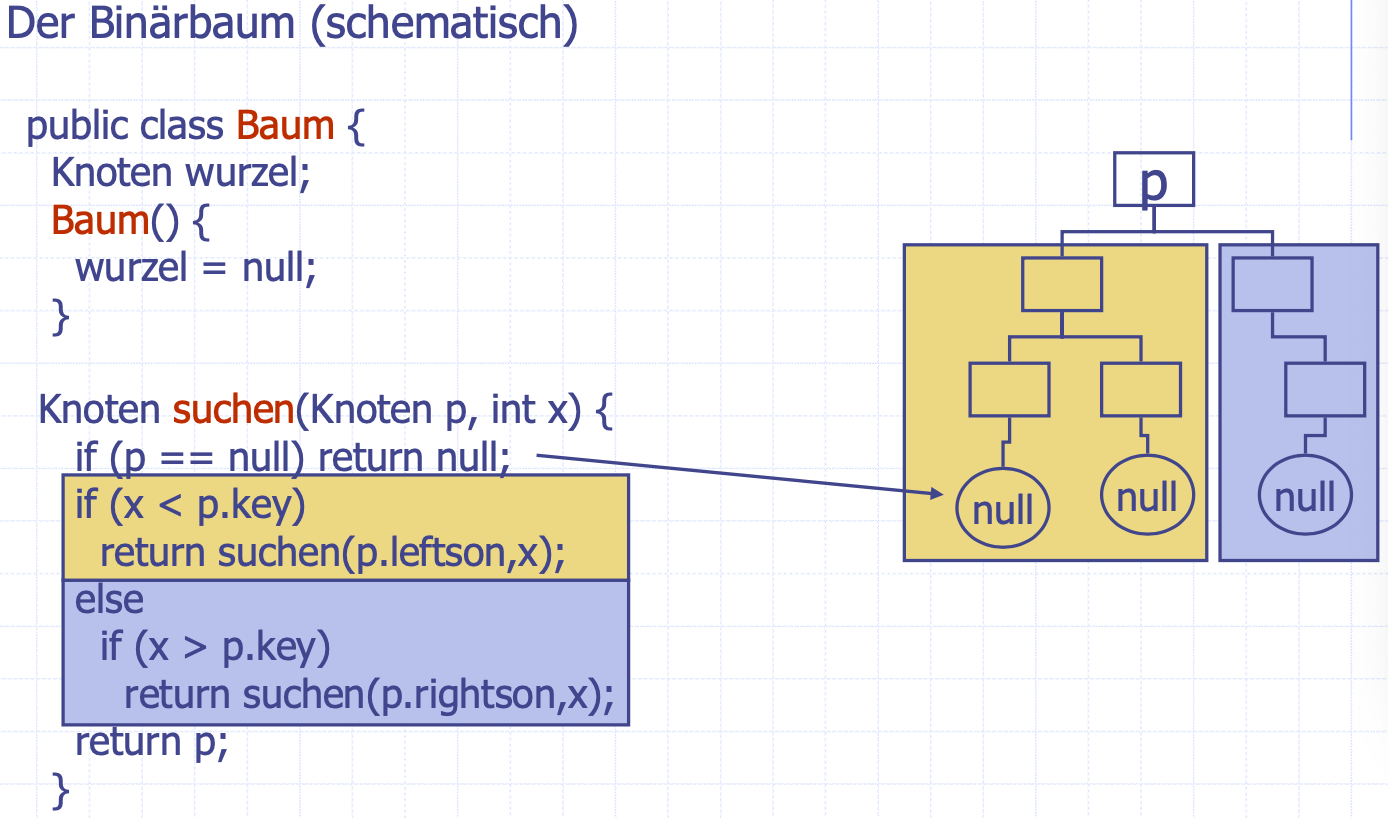
\includegraphics[scale=.22]{graphic/01 BinarySearchTrees/Baum.png}
\end{center}
\vspace{-8pt}

\subsubsection{einfügen}
\begin{center}
    \includegraphics[scale=.3]{graphic/01 BinarySearchTrees/einfügen.png}
\end{center}
\vspace{-12pt}

\subsubsection{entfernen}
\begin{center}
    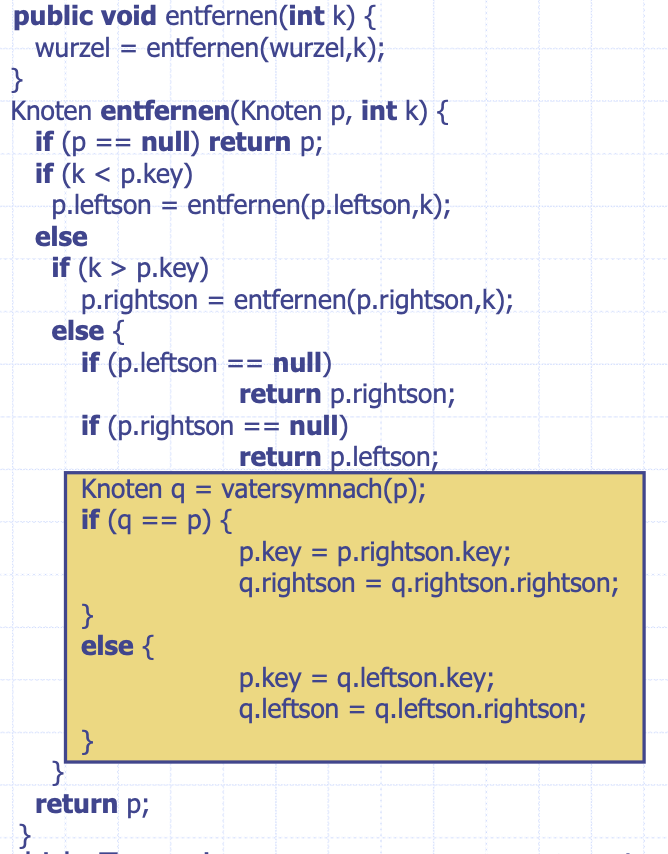
\includegraphics[scale=.3]{graphic/01 BinarySearchTrees/entfernen.png}
\end{center}
\vspace{-8pt}

\subsubsection{inorder}
\begin{center}
    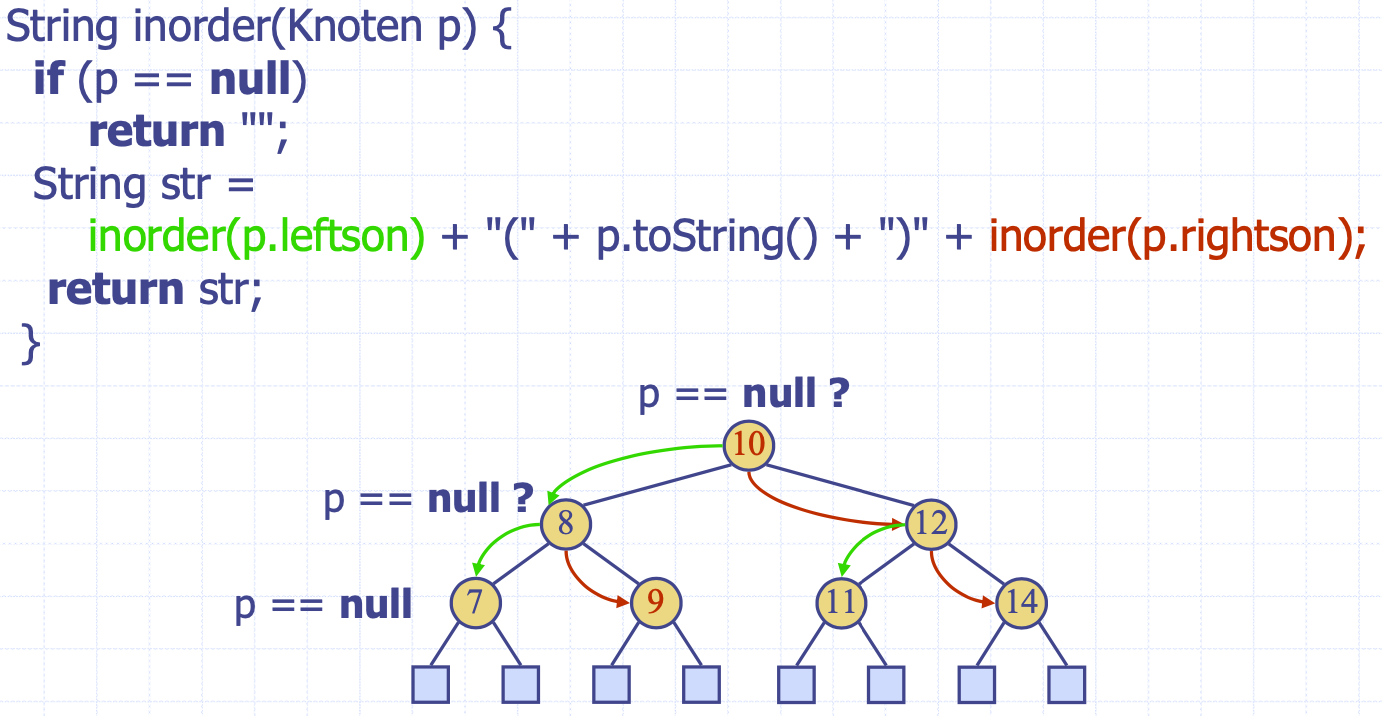
\includegraphics[scale=.22]{graphic/01 BinarySearchTrees/inorder().png}
\end{center}
\vspace{-8pt}




\newpage